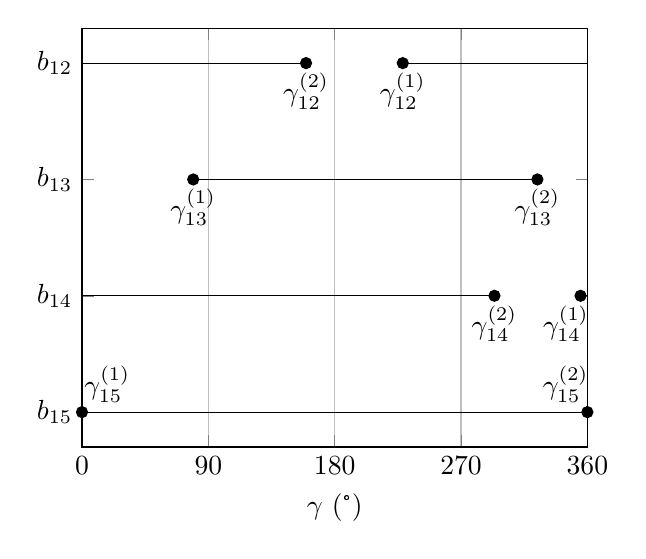
\begin{tikzpicture}
	\begin{axis}[width=8cm,xlabel={$\gamma$ (\textdegree)}, xtick={0,90,180,270,360}, xmin=0, xmax=360, ytick={1,...,4}, yticklabels={$b_{15}$,$b_{14}$,$b_{13}$,$b_{12}$},xmajorgrids]
	% Bogenspuren mit Kreis C_2
	\addplot[mark=*] plot coordinates  { (228.49,4) (370,4) } node[below, pos=0] {$\gamma^{(1)}_{12}$} ;
	\addplot[mark=*] plot coordinates { (-10,4) (159.59,4) } node[below, pos=1] {$\gamma^{(2)}_{12}$};
	
	% Bogenspuren mit Kreis C_3
	\addplot[mark=*] plot coordinates { (79.22,3) (324.38,3) } node[below, pos=0] {$\gamma^{(1)}_{13}$} node[below, pos=1] {$\gamma^{(2)}_{13}$};
	
	% Bogenspuren mit Kreis C_4
	\addplot[mark=*] plot coordinates { (355.12,2) (370,2) } node[below, pos=-.7] {$\gamma^{(1)}_{14}$};
	\addplot[mark=*] plot coordinates { (-10,2) (293.81,2) } node[below, pos=1] {$\gamma^{(2)}_{14}$};
	
	% Bogenspuren mit Kreis C_5
	\addplot[mark=*] plot coordinates { (0,1) (360,1) } node[above, pos=0.05] {$\gamma^{(1)}_{15}$} node[above, pos=0.957] {$\gamma^{(2)}_{15}$};
	
	% Füge noch eine graue Box zur Kennzeichnung der übriggebliebenen Bogenstücken hinzu
%	\fill [gray!60,fill opacity=0.2] (axis cs:79.22,1) rectangle (axis cs:159.59,4);
%	\fill [gray!60,fill opacity=0.2] (axis cs:228.49,1) rectangle (axis cs:293.81,4);
	\end{axis}
\end{tikzpicture}